\chapter{Number 1}
\section{Integers}
An integer is just a whole number, it does not have digits after the decimal point and it is not a fraction.  Early mathematics used some of these number to solve the kinds of problems that were important to the people of the day, like counting sheep or the number of days etc.
\section{Four Rules}
\subsection{Additition}
When we want to add two and three digit numbers together we follow an algorithm, a set of instructions.  If we follow these instructions correctly we will end up with the desired result.  Let's look at an algorithm for adding two numbers together.  We will first look at it displayed as a flow chart and then given as a series of steps:

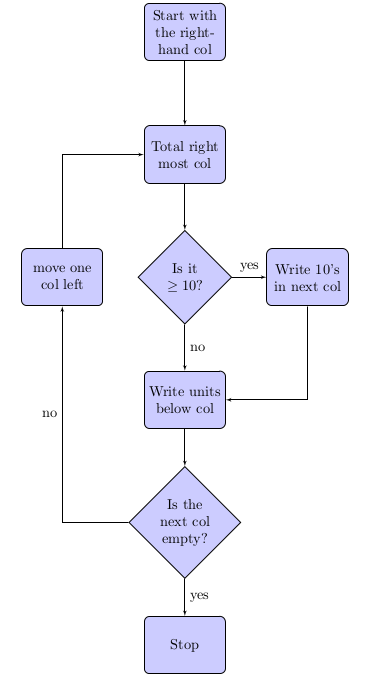
\includegraphics[width=15cm,height=15cm,keepaspectratio]{./Images/Number/Flow1}

\begin{enumerate}
	\item Write down the numbers lining up the digits by place value (i.e. units under units)
	\item Find the total of the right most column that has not already been totaled
	\item If the total is $> 10$ then write the tens part in the next column to the left
	\item Write down the units value
	\item If the next column is empty. STOP
	\item Go to step 2.
\end{enumerate}

\begin{exmp}
What is $256+28$?
Step 1. Write the numbers down, lining up the columns.

\renewcommand{\arraystretch}{1}
\begin{tabular}{c c c}
	2 & 5 & 6 \\
	  & 2 & 8 \\
	\hline \hline
	  &   &   \\
\end{tabular}

The right-hand column has a total of 14, that is 1 ten and 4 units.  We will now put the 1 in the next column and the 4 below the column we have just totaled.

\renewcommand{\arraystretch}{1}
\begin{tabular}{c c c}
	2 & 5 & 6 \\
	  & 2 & 8 \\
	\hline \hline
	  & $^1$  & 4 \\
\end{tabular}
\end{exmp}

The next column is not empty so let's find its total.
The total is 8 (don't forget the 1), so we have nothing to put in the next column, just 8 in this one.

\renewcommand{\arraystretch}{1}
\begin{tabular}{c c c}
	2 & 5 & 6 \\
	  & 2 & 8 \\
	\hline \hline
	  & $8^1$  & 4  \\
\end{tabular}

The next column is not empty so let's find its total.
The total is 2, so we have nothing to put in the next column, just 2 in this one.

\renewcommand{\arraystretch}{1}
\begin{tabular}{c c c}
	2 & 5 & 6 \\
	  & 2 & 8 \\
	\hline \hline
	2  & $8^1$  & 4  \\
\end{tabular}

The next column is empty so we have finished.  The answer is 284.
\subsection{Exercise}
Find the answers to the questions below, do not use a calculator:
\begin{multicols}{2}
\begin{enumerate}
  \item $45 + 28$
  \item $295 + 21$
  \item $462 + 352$
  \item $652 + 347$
  \item $147 + 345 + 252$
  \item $359 + 875$
  \item What is the total cost of a car at \$3457 and a boat at \$5385?
  \item What is the cost of a dog at \$299 and a cat at \$145?
  \item How much would it cost for a \$45 hat a \$72 shirt and a \$164 coat?
  \item The flight for a holiday is \$572 and the accomodation is \$365.  What is the total price?
  \item One boy has 864\cent \hspace{1 mm} and another has 395\cent, how much have they got in total?
  \item Fred has 28 apples, Timmy has 110 tomatoes and Steve has 2247 pears. How many fruits do they have altogether? (A.T.)
  \item A flight to Hong Kong costs \$396 per child, \$626 per adult and \$530 per student. How much would it cost for 2 adults, a child and a student to fly to Hong Kong? (I.F.)
  \item Frank wants to buy a \$39 pair of trousers a \$72 jacket and a \$16 burrito for lunch. How much is that in total? (C.C.S.)
  \item If you ate a slice of pizza that weighed 758 grams and a cookie that weighed 425 grams how much would you have eaten. (J.P.)
  \item How much would it cost if 100 doughnuts are \$245 and 80 waffles are \$193? (P.O.B.)
  \item What is the total cost of a mohawk haircut at \$53 and red hair dye at \$168? (L.G.)
  \item Jeboris spent \$4378 on a car and then \$950 on a new phone, how much did he spend in total? (J.L.)
  \item If Bill was in an aeroplane that travelled up 1874 metres and then another 297 metres, how far up would he be? (I.B.)
  \item Billy won a lotto of \$186944 in march. Later in April billy won a lotto of \$794999.  How much money would billy have if he combined all his lotto money together? (A.S)
\end{enumerate}
\end{multicols}
\subsection{Subtraction}
To subtract one number from another we can again follow an algorithm, but first we must learn how to \textbf{decompose/recompose} a number.
\noindent Let's consider the number $3053$ and look at all the different ways we can write it that will be useful for subtraction.

\renewcommand{\arraystretch}{1}
\begin{tabular}{| c | c | c | c |}
	\hline
	3 & 0 & 5 & 3 \\
	\hline
	3 & 0 & 4 & 13 \\
	\hline
	2 & 9 & 15 & 3 \\
	\hline
	2 & 10 & 5 & 3\\
	\hline
\end{tabular}

The first change makes the units column 10 bigger and the tens column 1 smaller.

The second change makes the tens column 10 bigger, but because the hundreds column is contains a zero we must make the number that makes up the thousands and hundreds columns 1 smaller.

The third change makes the hundreds column 10 bigger and the thousands column 1 smaller.

In each case we made the column to the right 10 bigger and the column, or if there were zeros present, columns to the left 1 smaller.

This technique will be important because we can only take a smaller number from a bigger one.

The algorithm
\begin{enumerate}
  \item Write down the two numbers lining up the digits
  \item Start at the right-hand column
  \item If the upper digit is larger than the lower digit then do the subtraction and write the number underneath
  \item If not, decompose/recompose the upper number so that the upper digit is 10 bigger
  \item move one column to the left
  \item repeat until the last column has been calculated
\end{enumerate}

\begin{exmp}
What is $342 - 227$?

\renewcommand{\arraystretch}{1}
\begin{tabular}{c c c}
	3 & 4 & 2 \\
	2 & 2 & 7 \\
	\hline \hline
	 & & \\
\end{tabular}

The 2 is smaller than the 7 so we will make it 10 bigger and the 4 we will make 1 smaller.

\begin{tabular}{c c c}
	3 & 3 & $^1 2$ \\
	2 & 2 & 7 \\
	\hline \hline
	 & & \\
\end{tabular}
We can now do the subtraction in this column.

\begin{tabular}{c c c}
	3 & 3 & $^1 2$ \\
	2 & 2 & 7 \\
	\hline \hline
	 & & 5\\
\end{tabular}

You should be able to see that we can now do the next two columns

\begin{tabular}{c c c}
	3 & 3 & $^1 2$ \\
	2 & 2 & 7 \\
	\hline \hline
	1 & 1 & 5\\
\end{tabular}

The the answer is 115.
\end{exmp}

\subsection{Exercise}
Find the answers to the questions below, do not use a calculator:
\begin{multicols}{2}
\begin{enumerate}
  \item $45 - 28$
  \item $295 - 21$
  \item $462 - 356$
  \item $652 - 347$
  \item $305 - 258$
  \item $914 - 655$
  \item A car on an online auction site costs \$658, we have \$894.  If we buy the car how much money will we have left?
  \item If one tree if 267cm tall and another is 385cm tall, what is the difference between their heights?
\end{enumerate}
\end{multicols}
\noindent The next few questions will require you use your understanding of previous sections of the book
\begin{enumerate}
	\setcounter{enumi}{8}
	\item Kite has 145\cent  \ and her brother has 372\cent.  If they put their money together and buy sweets costing 415\cent, how much change will they have?
	\item Esme has two pieces of wood, one 376cm long the other is 448cm long.  She wants to join them together to make a piece which is 525cm long  How much wood will she have left?
\end{enumerate}

\subsection{Multiplication}
There are many different algorithms that we can use to multiply two numbers together, in this book we will use the lattice method.  You might have another method that you prefer.

Let's show how this works by using an example.
\begin{exmp}
	What is $234 \times 56$?

	Since we are multiplying a three digit number by a two digit number we draw a 3 by 2 grid with the numbers lined up on the outside.

	\begin{center}
	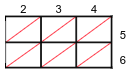
\includegraphics[height=2.1cm,keepaspectratio]{./Images/Number/mult1}
	\end{center}

	We start by treating our grid as a multiplication table.  Let's consider the last column and the bottom row ($4 \times 6$ which is $24$.  We put the ten's part (2) on the left side of the box and the unit's part (4) on the right side.

	\begin{center}
	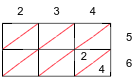
\includegraphics[height=2.1cm,keepaspectratio]{./Images/Number/mult2}
	\end{center}

	Let's fill out the rest of grid.

	\begin{center}
	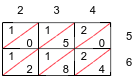
\includegraphics[height=2.1cm,keepaspectratio]{./Images/Number/mult3}
	\end{center}

	We now add up the values in each diagonal carry tens if required to get our answer.

	\begin{center}
	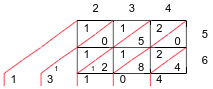
\includegraphics[height=2.5cm,keepaspectratio]{./Images/Number/mult4}
	\end{center}
\end{exmp}

\subsection{Exercise}
Find the answers to the questions below, do not use a calculator:
\begin{multicols}{2}
\begin{enumerate}
  \item $234 \times 55$
  \item $103 \times 27$
  \item $502 \times 16$
  \item $8625 \times 61$
  \item $492 \times 222$
  \item $195 \times 195$
\end{enumerate}
\end{multicols}
\begin{enumerate}
	\setcounter{enumi}{6}
	\item What is the weight of 27 bags each weighing 375g?
	\item A year group has 117 students who are 13 years old and 156 who are 14 years old.  What is the combined number of years that they have lived?
\end{enumerate}
\noindent The next few questions will require you use your understanding of previous sections of the book
\begin{enumerate}
	\setcounter{enumi}{8}
	\item A lift can carry a total weight of 950kg.  If 13 women enter the lift with weights all around 69kg, how much stuff can they carry with them before the lift becomes dangerous?
	\item On a road trip Esm\'e drives 45km a day for 27 days and Alex then drives 107km a day for 11 days.  How far do they travel altogether?
\end{enumerate}

\subsection{Division}
There are many ways to divide one number into another, we will use the method of short division.  One big difference with division is that we work from the left-hand column rather than the right-hand side.  The skills that we will require are division of single digit numbers and finding the remainder.

Let's see how this works using an example.

\begin{exmp}
What is $375 \div 5$?

First we need to set up our calculation area.  The answer will go above the line.
\begin{center}
\begin{tabular}{c  C{0.4cm} C{0.4cm} C{0.4cm}}
\cline{2-4}
\multicolumn{1}{c|}
5 & 3 & 7 & 5 \\
\end{tabular}
\end{center}

Now we check to see how many 5's go into 3, the value in the first column.  The answer is 0 so that goes on the answer line and the remainder of 3 goes over to the next column. This changes the 7 to 37.
\begin{center}
\begin{tabular}{c  C{0.4cm} C{0.4cm} C{0.4cm}}
 & 0 &  & \\
\cline{2-4}
\multicolumn{1}{c|}
5 & 3 & $^3$7 & 5 \\
\end{tabular}
\end{center}
Now we check how many 5's go into 37, the value now in the second column.  The answer is 7 so that goes on the answer line and the remainder of 2 goes over to the next column.  This changes the 5 to 25.

\begin{center}
\begin{tabular}{c  C{0.4cm} C{0.4cm} C{0.4cm}}
 & 0 & 7 & \\
\cline{2-4}
\multicolumn{1}{c|}
5 & 3 & $^3$7 & $^2$5 \\
\end{tabular}
\end{center}

Finally we check to see how many 5's go into 25.  The answer is 5 and that goes on the answer line.  There is no remainder.
\begin{center}
\begin{tabular}{c  C{0.4cm} C{0.4cm} C{0.4cm}}
 & 0 & 7 & 5\\
\cline{2-4}
\multicolumn{1}{c|}
5 & 3 & $^3$8 & $^2$5 \\
\end{tabular}
\end{center}

So $375 \div 5 = 75$
\end{exmp}

\subsection{Exercise}
Find the answers to the questions below, do not use a calculator:
\begin{multicols}{2}
\begin{enumerate}
	\item $216 \div 6$
	\item $681 \div 3$
	\item $5475 \div 5$
	\item $18599 \div 7$
	\item $292 \div 4$
	\item $8532 \div 9$
\end{enumerate}
\end{multicols}
If when we have got past the last column we still have a remainder, that is what is left over after the division.
Find the remainder, if there is one for the questions below:
\begin{multicols}{2}
\begin{enumerate}
	\setcounter{enumi}{6}
	\item $1544 \div 7$
	\item $557 \div 8$
	\item $7632 \div 3$
	\item $5316 \div 9$
\end{enumerate}
\end{multicols}

\begin{enumerate}
	\setcounter{enumi}{10}
	\item $531645$ can be divided by $9$ with no remainder.  Change the order of the digits in $531645$ and see what the remainder is now.  What do you notice.
\end{enumerate}
\noindent The next few questions will require you use your understanding of previous sections of the book
\begin{enumerate}
	\setcounter{enumi}{11}
	\item A group of 25 friends decide to share their sweets, they have about 15 each.  When another five friends comes along they decide still share they equally between everyone.  About how many sweets does each friend recieve?
\end{enumerate}

\section{Directed numbers}
Numbers can be positive or negative, because we are using the sign we call them directed numbers.  Let's consider what happens when we add directed numbers together.  Imagine that you have two bank accounts, one of them has \$15 in it and the other has -\$10 dollars in it.  If we were to add these accounts together we would have one account with \$5 in it.  So when we added the negative 10, we just subtracted 10.

\bigskip

Rule 1: When we add a negative we subtract, so $a + -b$ becomes $a - b$

\bigskip

By using the same method above we can easily convince ourselves of rule two.

\bigskip

Rule 2: When we add a positive we add, so $a + +b$ becomes $a + b$

\bigskip

Rules 3 and 4 are wo do with when we subtract directed numbers.

Like before we have two accounts, one with \$15 and one with -\$10.  We know that we have \$5 over all.  Know let's take away the account with \$15 in it, we now have a total of -\$10.  So taking away a positive values was just like subtracting.

\bigskip

Rule 3: When we subtract a positive we subtract, so $a - +b$ becomes $a - b$

\bigskip

Now let's take away the account with -\$10 in it, our balance has go up to \$15.  So take away a negative is like adding.

\bigskip

Rule 4: When we subtract a negative we add, so $a - -b$ becomes $a + b$

\bigskip

An easy way to remember these rules is that if the two signs are the same we add, if they are different we subtract.

\begin{exmp}
Calculate the following:
\begin{enumerate}
	\item $8 + -5$
	\item $7 + +6$
	\item $3 - -7$
	\item $15 - +4$
\end{enumerate}

Answers:
\begin{enumerate}
	\item $8 + -5$ becomes $8 - 5 = 3$
	\item $7 + +6$ becomes $7 + 6 = 13$
	\item $3 - -7$ becomes $3 + 7 = 10$
	\item $15 - +4$ becomes $15 - 4 = 11$
\end{enumerate}
\end{exmp}

\subsection{Exercise}
Find the answers to the following:
\begin{multicols}{2}
\begin{enumerate}
	\item $5 + -1$
	\item $36 + -6$
	\item $17 + +3$
	\item $-1 + +10$
	\item $7 - -10$
	\item $25 - +8$
	\item $23 - -23$
	\item $5 - +12$
\end{enumerate}
\end{multicols}

We will now look at how to multiply and divide directed numbers.
The proofs of these rules will be given in a later algebra section.
The size of the number is calculated by multiply/dividing the number parts, we just use rules 5 and 6 to work out the sign of the answer.

\bigskip

Rule 5: When we multiply/divide to numbers together with the same sign the answer is positive.

\bigskip

Rule 6: When we multiply/divide to numbers together with different signs the answer is negative.

\bigskip

\begin{exmp}
\begin{enumerate}
	\item $-8 \times -5$
	\item $6 \times +4$
	\item $-4 \times +3$
	\item $9 \times -2$
\end{enumerate}

Answers:
\begin{enumerate}
	\item $-8 \times -5$, the answer is positive and $8 \times 5 = 40$ so we get 40
	\item $6 \times +4$, the answer is positive and $6 \times 4 = 24$ so we get 24
	\item $-4 \times +3$, the answer is negative and $4 \times 3 = 12$ so we get -12
	\item $9 \times -2$, the answer is negative and $9 \times 2 = 18$ so we get -18
\end{enumerate}
\end{exmp}

\subsection{Exercise}
Calculate the following:
\begin{multicols}{2}
\begin{enumerate}
	\item $-4 \times -6$
	\item $5 \times -5$
	\item $8 \times +3$
	\item $-13 \times -4$
	\item $4 \times -7$
	\item $-3 \times -9$
\end{enumerate}
\end{multicols}
\section{Factors}
The factors of a number are the whole numbers that divide into the number leaving no remainder.  So, for example, the factors of 10 are 1, 2, 5 and 10.  Again we will use an algorithm to find all the factors of a number.  This is important because it is easy to think that we have them all and to have missed some out.
The algorithm
Let's find the factors of some number N
We what to find all the ways of writing $a \times b = N$ where a and b are integers and $a < b$
\begin{enumerate}
	\item Start with $a=1$
	\item Let $b = N \div a$
	\item If b is a whole number write down $a \times b$
	\item Add 1 to a
	\item If a has already been written down, STOP you have all the factors.
	\item Goto step 2
\end{enumerate}

\begin{exmp}
Find the factors of 28

Try 1: so $1 \times 28$

Try 2: so $2 \times 14$

Try 3: Dividing by 3 leaves a remainder

Try 4: so $4 \times 7$

Try 5: Dividing by 5 leaves a remainder

Try 6: Dividing by 6 leaves a remainder

Try 7: We already have 7 so let's stop.

The factors in order of size are 1, 2, 4, 7, 14, 28

We could have written this as:

\begin{tabular}{c}
28 \\
\hline
$1 \times 28$ \\
$2 \times 14$ \\
$4 \times 7$ \\
\end{tabular}
\end{exmp}

\subsection{Exercise}
Find the factors all the numbers from 1 to 20.  Make a note of how many factors each one has.

\section{Multiples}
The multiples of a number are the values in its times table.  So since the first five values in the 3 times table are 3, 6, 9, 12, 15 then the first five multiples of 3 are 3, 6, 9, 12 and 15.
\begin{exmp}
Find the first four multiples of 7:

$1 \times 7 = 7$

$2 \times 7 = 14$

$3 \times 7 = 21$

$4 \times 7 = 28$

So the first four multiples of 7 are 7, 14, 21 and 28.
\end{exmp}
\begin{exmp}
What is the 10th multiple of 8.

$10 \times 8 = 80$

The 10th multiple of 8 is 80.
\end{exmp}
\subsubsection{Generating a sequence of multiples from a formula}
Let's consider the function $y=3x$
Now let $x$ = whole number values starting at 1.

\begin{tabular}{c|c}
x & y \\
\hline
1 & 3 \\
2 & 6 \\
3 & 9 \\
4 & 12
\end{tabular}

We can see that the y column has given us the multiples of 3.  So we could say that a formula for generating the multplies of 3 is $y=3x$.

\subsection{Exercise}
For the following numbers find the first five multiples, the formula for generating the multiples and the value of the $20^{th}$ multiple.

\begin{enumerate}
	\item 5
	\item 7
	\item 2
	\item 3
	\item 10
	\item 12
\end{enumerate}
\subsection{HCF and LCM}
The Highest Common Factor (HCF) of two numbers is the largest number that is a factor of both numbers.  The Lowest Common Multiple (LCM) of two numbers if the smallest number that is a multiple of both numbers.
\begin{exmp}
Find the HCF of 12 and 16

The factors of 12 are 1, 2, 3, 4, 6, 12

The factors of 16 are 1, 2, 4, 8, 16

The largest number that appears in each list is 4,

So the HCF of 12 and 16 is 4.
\end{exmp}
\begin{exmp}
Find the LCM of 12 and 15

We will work with the largest number.

Does 12 go into 15? No.

Does 12 go into 30? No.

Does 12 go into 45? No.

Does 12 go into 60? Yes.  So the LCM of 12 and 15 is 60.
\end{exmp}
\subsection{Exercise}
For each pair of numbers below find their HCF and LCM
\begin{enumerate}
	\item 6 and 8
	\item 10 and 15
	\item 6 and 9
	\item 12 and 10
	\item 5 and 7
	\item 10 and 20
	\item 4, 6 and 10
\end{enumerate}
Solve the following word problems using L.C.M. or H.C.F.
\begin{enumerate}
	\setcounter{enumi}{7}
	\item Isobel and Anuha are shelving books at a public library. Isobel shelves 5 books at a time, whereas Anuha shelves 6 at a time. If they end up shelving the same number of books, what is the smallest number of books each could have shelved?
	\item Sam and Rose are making emergency-preparedness kits to share with friends. They have 20 bottles of water and
12 cans of food, which they would like to distribute equally among the kits, with nothing left over. What is the greatest number of kits Sam and Rose can make?
	\item Kate has 16 blue marbles and 8 white ones. If she wants to place them in identical groups without any marbles left over, what is the greatest number of groups Kate can make?
	\item Lucas is making trail mix out of 18 bags of nuts and 9 bags of dried fruit. He wants each new portion of trail mix to be identical, containing the same combination of bags of nuts and bags of dried fruit, with no bags left over. What is the greatest number of portions of trail mix Lucas can make?
	\item Isabelle has swimming lessons every fifth day and diving lessons every third day. If she had a swimming lesson and a diving lesson on May 5, when will be the next date on which she has both swimming and diving lessons?
	\item To encourage public transportation, Nathaniel and Guiliana want to give some friends envelopes with bus tickets and train tickets in them. If they have 18 bus tickets and 12 train tickets to split equally among the envelopes, and want no tickets left over, what is the greatest number of envelopes Nathaniel and Guiliana can make?
\end{enumerate}
\section{Decimals}
\subsection{Addition and Subtraction}
To Add and subtract decimals we can use the same methods that we use for integers, all we need to do is make sure that we line up the decimal points in the question and the answer.
\subsection{Exercise}

Find the answers to the questions below (show your working), do not use a calculator:
\begin{multicols}{2}
\begin{enumerate}
	\item $23.6 + 34.2$
	\item $473.3 + 34.8$
	\item $345.5 - 152.3$
	\item $45.46 - 28.54$
	\item $68.46 + 23.35$
	\item $2.625 - 1.526$
	\item $35.6 + 3.56$
	\item $35.6 - 3.56$
	\item $123 + 35.2$
	\item $362 - 94.4$
\end{enumerate}
\end{multicols}
\begin{enumerate}
\setcounter{enumi}{10}
	\item A ball costs \$15.45 and we buy it with a \$20 note.  What is the change?
	\item An alloy is made of 35.9g of iron and 0.25g of tungsten.  What is the total weight?
\end{enumerate}
\subsection{Multiplication}
The important thing to remember when we are multipling decimals together is that the total number of digits after the decimal points in the question is equal to the number of digits after the decimal point in the answer.

So to calculate $23.4 \times 1.02$ we first calculate $234 \times 102$ using any pencil and paper method (23868).  Now since we have a total of three digits after the decimal points in the question we will have three in the answer, so the answer is $23.868$

\subsection{Exercise}
\begin{multicols}{2}
\begin{enumerate}
	\item $25.6 \times 7.4$
	\item $0.5 \times 0.7$
	\item $0.23 \times 0.96$
	\item $7.23 \times 6$
	\item $8.45 \times 75.3$
	\item $4.3 \times 5.34$
	\item $3.45 \times 8.2$
	\item $7.25 \times 0.8$
\end{enumerate}
\end{multicols}
\subsection{Division}
The only extra skill that we need when dividing decimals is that of multiplying by powers of 10 (10, 100, 1000, etc).  If we multiply by a power of 10 the digits stay the same but they move a number places compared to the decimal point equal to the number of zeros after the 1.

So, for example, $4.7 \times 10 = 47$ and $0.13 \times 100 = 13$

In each case here we have turned our decimal into an integer by matching the number of digits after the decimal point to the number of zeros after the 1.

\subsubsection{Method}
\begin{enumerate}
	\item Make sure the number we are dividing by is an integer.  If it is not multiply both numbers by a power of 10 big enough to make it so.
	\item Do the division in the same way as integer division.
	\item If the number we are dividing is a decimal we just have to line up the decimal point in the answer with the one in the question.
\end{enumerate}

So $235.6 \div 0.7 = 2356 \div 7$

\subsection{Exercise}
Calculate:
\begin{enumerate}
	\item $235.6 \div 8$
	\item $235.6 \div 0.8$
	\item $23.56 \div 0.8$
	\item $23.56 \div 0.08$
	\item $235.6 \div 0.08$
	\item $1 \div 7$ find the first 4 digits after the decimal point
	\item $0.053 \div 0.4$
	\item $15 \div 8$ continue until there are no remainders.
\end{enumerate}
\section{Fractions}
A fraction is a division.  It is not a coincidence that a division sign is a dot over a dot and a fraction is a number over a number.  A fraction is always an integer divided by an integer.

\subsection{Fractions to Decimals}
To change a fraction to a decimal we simply divide the numerator (top number) by the denominator (bottom number)
\begin{exmp}
	Change $\frac{4}{5}$ to a decimal.

	$\frac{4}{5} = 4 \div 5$

	$\frac{4}{5} = 0.8$
\end{exmp}
\begin{exmp}
	Change $\frac{3}{8}$ to a decimal.

	$\frac{3}{8} = 3 \div 8$

	$\frac{3}{8} = 0.375$
\end{exmp}
\subsection{Exercise}
Change the following fractions to decimals, you may use a calculator.
\begin{multicols}{3}
\begin{enumerate}
	\item $\frac{7}{8}$
	\item $\frac{3}{4}$
	\item $\frac{1}{2}$
	\item $\frac{2}{3}$
	\item $\frac{7}{10}$
	\item $\frac{1}{4}$
	\item $\frac{2}{7}$
	\item $\frac{5}{7}$
	\item $\frac{6}{7}$
	\item $\frac{1}{9}$
	\item $\frac{2}{9}$
	\item $\frac{3}{9}$
	\item $\frac{4}{9}$
	\item $\frac{5}{9}$
	\item $\frac{6}{9}$
	\item $\frac{7}{9}$
	\item $\frac{8}{9}$
	\item $\frac{9}{9}$
\end{enumerate}
\end{multicols}
\subsection{Equivalent Fractions and simplifying fractions}
Equivalent fractions are fractions that when changed to decimals give exactly the same value.  So for example $\frac{2}{10}$ and $\frac{1}{5}$ give the same value of $0.2$ so these two fractions are equivalent.  To find a fraction that is equivalent to another you can simply multiply or divide the numerator and denominator by the same value, however, you must ensure that the new numerator and denominator are still integers.

\begin{exmp}
Find an equivalent fraction to $\frac{2}{7}$.

We can pick any integer value and multiply both parts of the fraction by that value.  I will pick '3'.

So the new equivalent fraction is $\frac{2 \times 3}{7 \times 3} = \frac{6}{21}$
\end{exmp}

When we talk about simplifying fractions we are talking about finding the equivalent fraction that consists of the lowest values.  The quickest way of doing this is by finding the numbers HCF and dividing both numbers by this value.  You can also just keep finding equivalent fractions where the values of both parts get smaller by dividing them by common values and then stopping when you can't divide any more.  Of course there is no point in dividing by '1'.

\begin{exmp}
	Simplify $\frac{18}{24}$

	Let's divide both numbers by 2.  We get $\frac{9}{12}$

	Let's divide both numbers by 3.  We get $\frac{3}{4}$

	Since the two numbers no longer have a common factor the simliest form of the fraction is $\frac{3}{4}$.

	Alternatively.

	The HCF of 18 and 24 is 6.  So we can get the simpliest form immediately by dividing both values by 6.
\end{exmp}

\subsection{Exercise}
For each fraction below find an equivalent fraction and where possible write the fraction in its simpliest form.
\begin{multicols}{3}
\begin{enumerate}
	\item $\frac{4}{6}$
	\item $\frac{20}{30}$
	\item $\frac{9}{15}$
	\item $\frac{25}{35}$
	\item $\frac{12}{24}$
	\item $\frac{42}{63}$
\end{enumerate}
\end{multicols}
\subsection{Changing a Mixed fraction to a top heavy fraction}
We will often see a number written like $\displaystyle 2 \frac{3}{5}$.  This is quite easy for us to understand, we have 2 whole parts and a fractional part of $\frac{3}{5}$.  However, when we are working with fractions it is usually best to only have a numerator and denominator.  In this section I will show you how to change $\displaystyle 2 \frac{3}{5}$ into the more useful $\displaystyle \frac{13}{5}$.  To do this we need to understand that if we have a denominator of size 'n' then we need 'n' of them to make a whole.  This is just like us needing 2 halfs to make a whole.

Let's look at $\displaystyle 2 \frac{3}{5}$

\bigskip

\noindent We can see that we are deal with fifths since that is the denominator.  We need to change our 2 into fifths.  Since 1 whole needs 5 fifths it follows that 2 whole will require twice as many, so we have $\frac{10}{5}$ and $\frac{3}{5}$ that is a total $\frac{13}{5}$

\noindent You might have noticed that the denominator did not change and that we just multiplied the whole part by the denominator and added the numerator.  We can write this as:\bigskip

$\displaystyle a \frac{b}{c} = \frac{a \times c + b}{c}$

\begin{exmp}
Write $\displaystyle 3 \frac{2}{7}$ as a top heavy fraction.\bigskip

$\displaystyle 3 \frac{2}{7} = \frac{3 \times 7 + 2}{7}$

\bigskip

$\displaystyle 3 \frac{2}{7} = \frac{23}{7}$\bigskip
\end{exmp}
\subsection{Exercise}
Write the following mixed fractions as top heavy fractions.
\begin{multicols}{3}
\begin{enumerate}
	\item $\displaystyle 1 \frac{1}{2}$
	\item $\displaystyle 2 \frac{3}{5}$
	\item $\displaystyle 2 \frac{4}{7}$
	\item $\displaystyle 5 \frac{1}{2}$
	\item $\displaystyle 4 \frac{2}{3}$
	\item $\displaystyle 3 \frac{3}{10}$
	\item $\displaystyle 2 \frac{5}{6}$
	\item $\displaystyle 3 \frac{4}{5}$
	\item $\displaystyle 4 \frac{2}{5}$
\end{enumerate}
\end{multicols}

\subsection{Changing a top heavy fraction into a mixed fraction}
In this section we will learn how to perform tasks like changing $\displaystyle \frac{17}{3}$ into $\displaystyle 5 \frac{2}{3}$

\bigskip

Since the denominator does not change and we now know how many of this type of fraction are required to create one whole all we need to do is calculate how many of the denominators divide into the numerator and its remainder.

Let's consider $\displaystyle \frac{17}{3}$

\bigskip

3 goes into 17 five times.  That means we can create 5 wholes, which uses 15 of the $\frac{1}{3}$'s.  We have 2 $\frac{1}{3}$'s more. So the answer is: \bigskip

$\displaystyle \frac{17}{3} = 5 \frac{2}{3}$

\begin{exmp}
Write $\displaystyle \frac{23}{5}$ as a mixed fraction. \bigskip

5 goes into 23, 4 times with a remainder of 3. So: \bigskip

$\displaystyle \frac{23}{5} = 4 \frac{3}{5}$
\end{exmp}

\subsection{Exercise}
Write the following top heavy fractions as mixed fractions.
\begin{multicols}{3}
\begin{enumerate}
	\item $\displaystyle \frac{18}{5}$
	\item $\displaystyle \frac{15}{4}$
	\item $\displaystyle \frac{9}{2}$
	\item $\displaystyle \frac{16}{7}$
	\item $\displaystyle \frac{28}{11}$
	\item $\displaystyle \frac{18}{8}$
	\item $\displaystyle \frac{25}{10}$
	\item $\displaystyle \frac{11}{4}$
	\item $\displaystyle \frac{19}{6}$
\end{enumerate}
\end{multicols}

\subsection{Multiplying a fraction by an integer}
We can think of a fraction as the denominator specifying the size an individual item and the numerator specifying how many we have.  So, for instance, $\frac{3}{5}$ could mean that the size of an item is a fifth and we have three of them.
So if we were to multiply $\frac{3}{5}$ by 4 we would no longer have 3 fifths we would now have 12 fifths.
So we can see that when we multiply a fraction by an integer we just have to multiply the numerator by the integer.
\begin{exmp}
What is $\frac{2}{7} \times 3$?

Ans. $\frac{2 \times 3}{7} = \frac{6}{7}$
\end{exmp}

We could write this as $\displaystyle\frac{a}{b} \times c = \frac{a \times c}{b}$

\subsection{Exercise}
Find the value of the following multiplications
\begin{enumerate}
	\item $\frac{5}{7} \times 4$
	\item $\frac{1}{6} \times 3$
	\item $\frac{2}{9} \times 5$
	\item $\frac{3}{5} \times 3$
	\item $2 \times \frac{1}{9}$
	\item $5 \times \frac{3}{4}$
	\item $7 \times \frac{5}{8}$
	\item $10 \times \frac{5}{6}$
\end{enumerate}

\subsection{Multiplying a fraction by another fraction which has a numerator of 1}
Let's consider an example.

$\displaystyle \frac{1}{3} \times \frac{5}{7}$

\noindent We can write this as $\displaystyle \frac{1}{3}$ of $\displaystyle \frac{5}{7}$

We should be able to understand that if we have a third as much then size of the pieces is three times smaller.  Therefore, we need to make the denominator three times bigger.

As a result of the above argument we can see that when calculating this type of problem we multiply the denominators together.

\begin{exmp}
Calculate $\displaystyle \frac{1}{5} \times \frac{3}{4}$

$\displaystyle \frac{1}{5} \times \frac{3}{4} = \frac{3}{5 \times 4}$

So

$\displaystyle \frac{1}{5} \times \frac{3}{4} = \frac{3}{20}$
\end{exmp}

We could write this as $\displaystyle\frac{1}{a} \times \frac{b}{c} = \frac{b}{a \times c}$

\subsection{Exercise}
Find the value of the following multiplications
\begin{enumerate}
	\item $\frac{1}{7} \times \frac{3}{7}$
	\item $\frac{1}{6} \times \frac{5}{7}$
	\item $\frac{1}{2} \times \frac{3}{11}$
	\item $\frac{1}{5} \times \frac{1}{5}$
	\item $\frac{1}{8} \times \frac{3}{8}$
	\item $\frac{1}{5} \times \frac{2}{7}$
	\item $\frac{1}{3} \times \frac{3}{5}$
	\item $\frac{1}{9} \times \frac{3}{4}$
\end{enumerate}

\section{Four Rules}
\subsection{Multiplying two fractions together}
It can be seen from the previous two sections that if we wish to multiply two fractions together we simply multiply the numerators together and the denominators together.

So $\displaystyle \frac{a}{b} \times \frac{c}{d} = \frac{a \times c}{b \times d}$

\begin{exmp}
Calculate $\displaystyle \frac{3}{11} \times \frac{2}{9}$

\bigskip

$\displaystyle \frac{3}{11} \times \frac{2}{9} = \frac{3 \times 2}{11 \times 9}$

\bigskip

$\displaystyle \frac{3}{11} \times \frac{2}{9} = \frac{6}{99}$

\bigskip

\noindent We can see that this faction can be simplified, so we will divide the numerator and denominator both by 3.

\bigskip

$\displaystyle \frac{3}{11} \times \frac{2}{9} = \frac{2}{33}$

\bigskip

\noindent In the next example we will see how we could have simplified within the question instead.
\end{exmp}

\begin{exmp}
Calculate $\displaystyle \frac{3}{5} \times \frac{5}{9}$

\bigskip

\noindent Because when we multiply to integers together the order does not matter, it means that we can simpify fractions in the questions by finding values that will divide into any number in the numerator with any number in the denominator.

We can see here that 5 will divide into both 5's to give:\bigskip

$\displaystyle \frac{3}{5} \times \frac{5}{9} = \frac{3}{1} \times \frac{1}{9}$

\bigskip

We can also see that 3 divides into 3 and 9 to give:\bigskip

$\displaystyle \frac{3}{1} \times \frac{1}{9} = \frac{1}{1} \times \frac{1}{3}$

\bigskip

So the answer is:\bigskip

$\displaystyle \frac{3}{5} \times \frac{5}{9} = \frac{1}{3}$
\end{exmp}
\subsection{Exercise}
Work out the following questions without using a calculator.  Check to see if you can simplify your answer.
\begin{multicols}{2}
\begin{enumerate}
	\item $\displaystyle \frac{2}{3} \times \frac{4}{5}$
	\item $\displaystyle \frac{3}{5} \times \frac{1}{4}$
	\item $\displaystyle \frac{5}{9} \times \frac{2}{7}$
	\item $\displaystyle \frac{2}{3} \times \frac{1}{4}$
	\item $\displaystyle \frac{3}{8} \times \frac{2}{9}$
	\item $\displaystyle \frac{2}{3} \times \frac{2}{3}$
	\item $\displaystyle \frac{4}{9} \times \frac{2}{5}$
	\item $\displaystyle \frac{1}{3} \times \frac{4}{15}$
	\item $\displaystyle \frac{2}{5} \times \frac{5}{6} \times \frac{3}{7}$
	\item $\displaystyle \frac{1}{2} \times \frac{2}{3} \times \frac{3}{4}$
\end{enumerate}
\end{multicols}
\subsection{Dividing Fractions}
We will show why this works in a later algebra section of the book.  For now we will just learn that we can change a division question into a multiplication question by inverting the fraction after the division sign.

\begin{exmp}
Change $\displaystyle \frac{1}{3} \div \frac{4}{5}$ into a multiplication.

\bigskip

So we will change the $\div$ into a $\times$ and invert the fraction after the $\div$

\bigskip

$\displaystyle \frac{1}{3} \div \frac{4}{5} = \frac{1}{3} \times \frac{5}{4}$

\bigskip

The result would be $\displaystyle \frac{5}{12}$
\end{exmp}

\subsection{Exercise}
Work out the following questions without using a calculator.  Check to see if you can simplify your answer, you do not need to change top heavy fractions into mixed fractions.
\begin{multicols}{2}
\begin{enumerate}
	\item $\displaystyle \frac{2}{3} \div \frac{4}{5}$
	\item $\displaystyle \frac{3}{5} \div \frac{1}{4}$
	\item $\displaystyle \frac{5}{9} \div \frac{2}{7}$
	\item $\displaystyle \frac{2}{3} \div \frac{1}{4}$
	\item $\displaystyle \frac{3}{8} \div \frac{2}{9}$
	\item $\displaystyle \frac{2}{3} \div \frac{2}{3}$
	\item $\displaystyle \frac{4}{9} \div \frac{2}{5}$
	\item $\displaystyle \frac{1}{3} \div \frac{4}{15}$
	\item $\displaystyle \frac{2}{5} \times \frac{5}{6} \div \frac{3}{7}$
	\item $\displaystyle \frac{1}{2} \times \frac{2}{3} \div \frac{3}{4}$
\end{enumerate}
\end{multicols}

\subsection{Adding and subtracting fractions with the same denominator}
Since the denominator tells us what kind of fraction we are dealing with and the numerator informs us of how many we have, the process of adding or subtracting fractions only requires us add or subtract the numerators.
\bigskip

\noindent So we can write this as $\displaystyle \frac{a}{b} \pm \frac{c}{b} = \frac{a \pm c}{b}$

\begin{exmp}
	Calculate $\displaystyle \frac{2}{7} + \frac{3}{7}$

	\bigskip

	$\displaystyle \frac{2}{7} + \frac{3}{7} = \frac{2 + 3}{7}$

	\bigskip

	So

	\bigskip

	$\displaystyle \frac{2}{7} + \frac{3}{7} = \frac{5}{7}$
\end{exmp}

\begin{exmp}
	Calculate $\displaystyle \frac{5}{9} - \frac{1}{9}$

	\bigskip

	$\displaystyle \frac{5}{9} - \frac{1}{9}= \frac{5 - 1}{9}$

	\bigskip

	So

	\bigskip

	$\displaystyle \frac{5}{9} - \frac{1}{9}= \frac{4}{9}$
\end{exmp}

\begin{exmp}
	Calculate $\displaystyle 2 \frac{3}{11} + \frac{3}{11}$

	\bigskip

	First we need to change the mixed fraction into a top heavy fraction.

	\bigskip

	$\displaystyle 2 \frac{3}{11} + \frac{3}{11} = \frac{25}{11} + \frac{3}{11}$

	\bigskip

	So

	\bigskip

	$\displaystyle 2 \frac{3}{11} + \frac{3}{11} = \frac{28}{11}$
\end{exmp}

\subsection{Exercise}
Calculate the following and simplify if possible:
\begin{multicols}{2}
\begin{enumerate}
	\item $\displaystyle \frac{3}{8} + \frac{1}{8}$
	\item $\displaystyle \frac{4}{5} - \frac{1}{5}$
	\item $\displaystyle 3 \frac{2}{7} + \frac{2}{7}$
	\item $\displaystyle 2 \frac{4}{9} - \frac{7}{9}$
	\item $\displaystyle \frac{3}{8} + \frac{3}{8}$
	\item $\displaystyle \frac{5}{8} + \frac{1}{8} + \frac{7}{8}$
\end{enumerate}
\end{multicols}

\subsection{Adding and subtracting fractions with the different denominators}
We have seen how to add fractions which have the same denominator, but what do we do if the denominators are different.  Well we use our knowledge of equivalent fractions to make the denominators the same.  We can do this by multiplying the numerator and denominator of each fraction by the other fractions denominator.

\bigskip

\noindent Consider $\displaystyle \frac{2}{5} + \frac{1}{3}$

\bigskip

\noindent Here we would multiply the numerator and denominator of the first fraction by 3 and the numerator and denominator of the second fraction by 5.  Now we have two fractions both with a denominator of 15.

\begin{exmp}
	Calculate $\displaystyle \frac{3}{8} + \frac{2}{5}$

	\bigskip

\noindent We will multiply the numerator and denominator of the first fraction by 5 and the numerator and denominator of the second fraction by 8.

\noindent So

	\bigskip

	$\displaystyle \frac{3}{8} + \frac{2}{5} = \frac{15}{40} + \frac{16}{40}$

	\bigskip

\noindent So

	\bigskip

	$\displaystyle \frac{3}{8} + \frac{2}{5} = \frac{31}{40}$
\end{exmp}

\subsection{Exercise}
Calculate the following and simplify if possible:
\begin{multicols}{2}
\begin{enumerate}
	\item $\displaystyle \frac{3}{8} + \frac{1}{5}$
	\item $\displaystyle \frac{4}{9} - \frac{1}{5}$
	\item $\displaystyle 3 \frac{2}{7} + \frac{2}{9}$
	\item $\displaystyle 2 \frac{4}{9} - \frac{7}{11}$
	\item $\displaystyle \frac{3}{8} + \frac{3}{5}$
	\item $\displaystyle \frac{2}{9} + \frac{1}{4}$
\end{enumerate}
\end{multicols}
